\documentclass{article}
\usepackage{latexsym}
\usepackage{amssymb}
\usepackage{graphicx}
\usepackage{gensymb}
\usepackage[margin=1.2in]{geometry}
\usepackage{float}
\usepackage{wrapfig}
\usepackage{amsthm}
\usepackage{blkarray}
\usepackage{amsmath}
\usepackage{mathtools}
\usepackage{tikz}

\usepackage{framed}
\usepackage{fancyhdr}
\setcounter{page}{0}
\fancypagestyle{plain}{%
\pagestyle{fancy}
\fancyhf{}
\rhead{Tom Goodman}
\lhead{\leftmark}
\chead{Introduction to AI - Exercise II}
\cfoot{\thepage} 
\renewcommand{\footrulewidth}{2pt}}
\pagestyle{plain}
\newcounter{thrmcount}[section]

\usepackage{graphicx}
    \graphicspath{ {/home/txg523/Desktop/Tex} }
    
\usepackage{hhline}

\newenvironment{thrm}
	{\begin{leftbar}\noindent\ignorespaces\textbf{Theorem \arabic{section}.\arabic{thrmcount}.}\par\noindent\ignorespaces}		
	{\end{leftbar}\stepcounter{thrmcount}\noindent\ignorespaces}
\newenvironment{lem}
	{\begin{leftbar}\noindent\ignorespaces\textbf{Lemma \arabic{section}.\arabic{thrmcount}.}\par\noindent\ignorespaces}		
	{\end{leftbar}\stepcounter{thrmcount}\noindent\ignorespaces}
\newenvironment{nthrm}[1]	
	{\begin{leftbar}\noindent\ignorespaces\textbf{Theorem \arabic{section}.\arabic{thrmcount}.} \textit{(#1)}\par\noindent\ignorespaces}
	{\end{leftbar}\stepcounter{thrmcount}\noindent\ignorespaces}
\newenvironment{nlem}[1]
	{\begin{leftbar}\noindent\ignorespaces\textbf{Lemma \arabic{section}.\arabic{thrmcount}.} \textit{(#1)}\par\noindent\ignorespaces}
	{\end{leftbar}\stepcounter{thrmcount}\noindent\ignorespaces}
\newenvironment{defn}
	{\begin{leftbar}\noindent\ignorespaces\textbf{Definition.}\par\noindent\ignorespaces}
	{\end{leftbar}\noindent\ignorespaces}
\newenvironment{nproof}
	{\begin{proof}}
	{\newline\end{proof}\noindent\ignorespaces}
\newenvironment{prop}
	{\begin{leftbar}\noindent\ignorespaces\textbf{Proposition \arabic{section}.\arabic{thrmcount}.}\par\noindent\ignorespaces}		
	{\end{leftbar}\stepcounter{thrmcount}\noindent\ignorespaces}
\newenvironment{fact}
	{\begin{leftbar}\noindent\ignorespaces\textbf{Fact \arabic{section}.\arabic{thrmcount}.}\par\noindent\ignorespaces}		
	{\end{leftbar}\stepcounter{thrmcount}\noindent\ignorespaces}
\newenvironment{crl}
	{\begin{leftbar}\noindent\ignorespaces\textbf{Corollary \arabic{section}.\arabic{thrmcount}.}\par\noindent\ignorespaces}		
	{\end{leftbar}\stepcounter{thrmcount}\noindent\ignorespaces}	
\newenvironment{ex}[1]
	{\begin{leftbar}\noindent\ignorespaces\textbf{Example.} (\textit{#1})\par\noindent\ignorespaces}
	{\end{leftbar}\noindent\ignorespaces}
\newenvironment{exa}
	{\begin{leftbar}\noindent\ignorespaces\textbf{Example.}\par\noindent\ignorespaces}
	{\end{leftbar}\noindent\ignorespaces}
\newcommand\ddfrac[2]{\frac{\displaystyle #1}{\displaystyle #2}}
\newcommand{\appropto}{\mathrel{\vcenter{
  \offinterlineskip\halign{\hfil$##$\cr
    \propto\cr\noalign{\kern2pt}\sim\cr\noalign{\kern-2pt}}}}}
\title{Introduction to AI - Exercise II}
\author{Tom Goodman}
\date{}
\begin{document}
\begin{titlepage}
	\begin{flushleft}
		\vspace*{1cm}
		\Huge
		\textbf{Introduction to AI - Exercise II} \\
		\vspace*{1cm}
		\Large
		\textbf{Tom Goodman} \\
	\end{flushleft}
\end{titlepage}
\newpage
\section{Question One}
\subsection{Brief}
\textit{Draw a semantic net that represents the following data:} $[20\%]$
\begin{center}
\textit{Tom is a cat. \\
Tom caught a bird. \\ 
Tom is owned by John. \\
Tom is ginger in colour. \\
Cats like cream. \\
The cat sat on the mat. \\
A cat is a mammal. \\ 
A bird is an animal. \\
All mammals are animals. \\
Mammals have fur.}
\end{center}

\subsection{Answer}
\begin{center}
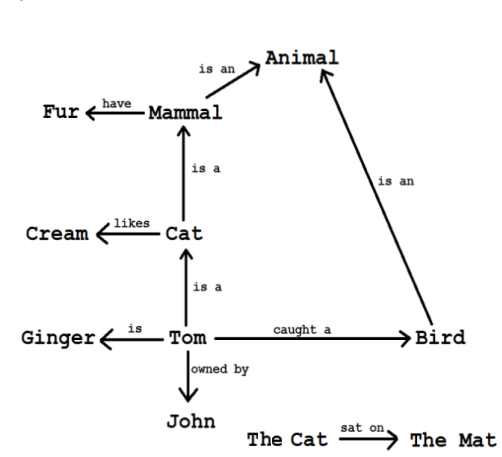
\includegraphics{IntroToAIE2SemanticWeb.png}
\end{center}
\newpage
\section{Question Two}
\subsection{Brief}
\textit{There are three hardware companies manufacturing graphics cards. The table below gives
the single joint probability distribution for the following two random variables:}
$[20\%]$ \\
\newline
\textit{(a) a card is good or defective, \\
(b) a card has been manufactured by company X.} 
\begin{center}
\begin{tabular}{cc || c | c}
\multicolumn{1}{c}{} & \multicolumn{1}{c}{} & \multicolumn{1}{c}{\textbf{G}} & \multicolumn{1}{c}{\textbf{D}} \\
$\ $ & \textit{Company} & \textit{Good} & \textit{Defective} \\ \hhline{~=#=|=}
\textbf{A} & \textit{Alf-Leiters} & 0.475 &  0.025 \\ \hhline{~-|-|-}
\textbf{B} & \textit{ Biodes $\&$ Son} & 0.279 & 0.021 \\ \hhline{~-|-|-}
\textbf{C} & \textit{Condictors Ltd.} & 0.180 & 0.020 \\
\end{tabular}
\end{center}
\textit{Consider the following questions: \\
\newline
(a) What is the market share of Alf-Leiters? \\ 
(b) What is the probability a randomly selected card is defective? \\
(c) What is the likelihood of Condictors Ltd. producing a defective card? \\
(d) What is the probability that a defective product came from Biodes $\&$ Son? \\
(e) Show whether or not the two events “Product is defective” and “Product is from
company X” are independent.
}
\subsection{Answer - (a)}
Market share of \textbf{A} is:
$$0.475 + 0.025 = 0.5$$

\subsection{Answer - (b)}
Randomly selected card is defective =
\begin{align*}
\sum\nolimits_{D_i} P(D), \ \ \ D_{i} &= (A_{D}, B_{D}, C_{D}) \\
&= 0.025 + 0.021 + 0.020 = 0.066
\end{align*}

\subsection{Answer - (c)}
Since we are finding the probability that the card is defective given that it was manufactured by company \textbf{C}, \\
$$P(D|C) = \ddfrac{P(D\cap C)}{P(C)}$$
$$P(D\cap C) = 0.020,\ which\ is\ the\ probability\ that\ it\ is\ defective\ and\ from\ company\ \textbf{C}.$$
$$P(C) = 0.180 + 0.020,\ which\ is\ the\ market\ share\ of\ \textbf{C}.$$
$$Hence,\ \ P(D|C) = \ddfrac{0.020}{0.200} = 0.1$$

\newpage
\subsection{Answer - (d)}
Since we are finding the probability that company \textbf{B} make the card, given that it is defective, \\
$$P(B|D) = \ddfrac{P(B\cap D)}{P(D)}$$
$$P(B\cap D) = 0.021\ which\ is\ the\ probability\ that\ it\ is\ defective\ and\ from\ company\ \textbf{B}.$$
$$P(D) = 0.066,\ (see\ Answer\ \textbf{(b)}).$$
$$Hence,\ \ P(B|D) = \ddfrac{0.021}{0.066} = \ddfrac{7}{22} \approx 0.\overline{318} $$

\subsection{Answer - (e)}
Two events, A and B, are independent iff $P(A\cap B) = P(A)P(B)$.
This means we need to test the following cases for independence:
$$P(D) \land P(A)$$
$$P(D) \land P(B)$$
$$P(D) \land P(C)$$

\begin{align*}
P(D\cap A) &= 0.025 \\
P(D)P(A) &= 0.066 \cdot 0.5 = 0.033
\end{align*}
Since $P(D\cap A) \neq P(D)P(A)$, the two are dependent.
\\

\begin{align*}
P(D\cap B) &= 0.021 \\
P(D)P(B) &= 0.066 \cdot 0.3 = 0.0198
\end{align*}
Since $P(D\cap B) \neq P(D)P(B)$, the two are dependent.
\\

\begin{align*}
P(D\cap C) &= 0.020 \\
P(D)P(C) &= 0.066 \cdot 0.2 = 0.0132 \\ 
\end{align*}
Since $P(D\cap C) \neq P(D)P(C)$, the two are dependent.
\\

Hence, the events "Product is defective" and "Product is from company X" are dependent.
 
\newpage
\section{Question 3}
\subsection{Brief}
\textit{
The following is a small planning problem, involving moving passengers using planes. The
predicates for the domain are: \\
\newline
at(Person, Airport), place(Airport), passenger(Person),
atPlane(Airport), emptyPlane, onPlane(Person), planeless(Airport)\\
\newline
The Strips operators are:\\
\newline
BOARD(X,Y) \\
\-\hspace{10mm} Preconditions: at(X,Y), place(Y), passenger(X), atPlane(Y), emptyPlane \\
\-\hspace{10mm} Delete List: at(X,Y), emptyPlane \\
\-\hspace{10mm} Add List: onPlane(X) \\
\newline
FLY(X,Y) \\
\-\hspace{10mm} Preconditions: atPlane(X), place(X), place(Y), planeless(Y) \\
\-\hspace{10mm} Delete List: atPlane(X), planeless(Y) \\
\-\hspace{10mm} Add List: atPlane(Y), planeless(X) \\
\newline
DISEMBARK(X,Y) \\
\-\hspace{10mm} Preconditions: onPlane(X), passenger(X), place(Y), atPlane(Y) \\
\-\hspace{10mm} Delete List:onPlane(X) \\
\-\hspace{10mm} Add List: at(X,Y), emptyPlane \\
\newline
Show how STRIPS would solve this planning problem using forward chaining for the
initial and goal state below. Assume that STRIPS always makes the correct choice.
Write down carefully all the intermediate states. $[30\%]$ \\
\newline
\textbf{Initial State}: place(bhx),
place(cdg), passenger(john), at(john,bhx), passenger(mary), at(mary, cdg), \\
atPlane(bhx), planeless(cdg), emptyPlane \\ \newline 
\textbf{Goal State}: at(john, cdg), at(mary, bhx)
}
\subsection{Answer}
place(bhx),
place(cdg), passenger(john), at(john,bhx), passenger(mary), at(mary, cdg), \\
atPlane(bhx), planeless(cdg), emptyPlane \\ 
\newline 
BOARD(john, bhx) \\
\-\hspace{10mm}  	- at(john, bhx) \\
\-\hspace{10mm}  	- emptyPlane \\
\-\hspace{10mm}  	+ onPlane(john) \\
\newline
place(bhx),
place(cdg), passenger(john), passenger(mary), at(mary, cdg), \\
atPlane(bhx), planeless(cdg), onPlane(john)\\ 
\newline
FLY(bhx, cdg) \\
\-\hspace{10mm} 	- atPlane(bhx) \\
\-\hspace{10mm} 	- planeless(cdg) \\
\-\hspace{10mm} 	+ atPlane(cdg) \\
\-\hspace{10mm} 	+ planeless(bhx) \\
\newline
place(bhx),
place(cdg), passenger(john), passenger(mary), at(mary, cdg), \\
onPlane(john), atPlane(cdg), planeless(bhx),\\ 
\newline
DISEMBARK(john, cdg) \\
\-\hspace{10mm} 	- onPlane(john) \\
\-\hspace{10mm} 	+ at(john, cdg) \\
\-\hspace{10mm} 	+ emptyPlane \\
\newline
place(bhx),
place(cdg), passenger(john), passenger(mary), at(mary, cdg), \\
atPlane(cdg), planeless(bhx), at(john, cdg), emptyPlane\\ 
\newline
BOARD(mary, cdg) \\
\-\hspace{10mm} 	- at(mary, cdg) \\
\-\hspace{10mm} 	- emptyPlane \\
\-\hspace{10mm} 	+ onPlane(mary) \\
\newline
place(bhx),
place(cdg), passenger(john), passenger(mary), atPlane(cdg), \\
planeless(bhx), at(john, cdg), onPlane(mary)\\ 
\newline
FLY(cdg, bhx) \\
\-\hspace{10mm} 	- atPlane(cdg) \\
\-\hspace{10mm} 	- planeless(bhx) \\
\-\hspace{10mm} 	+ atPlane(bhx) \\
\-\hspace{10mm} 	+ planeless(cdg) \\
\newline
place(bhx),
place(cdg), passenger(john), passenger(mary), at(john, cdg), \\
onPlane(mary), atPlane(bhx), planeless(cdg) \\
\newline
DISEMBARK(mary, bhx) \\
\-\hspace{10mm} - onPlane(mary \\
\-\hspace{10mm} + at(mary, bhx) \\
\-\hspace{10mm} + emptyPlane \\
\newline
place(bhx),
place(cdg), passenger(john), passenger(mary), at(john, cdg), \\
atPlane(bhx), planeless(cdg), at(mary, bhx), emptyPlane \\
\newpage
\section{Question 4}
\subsection{Brief}
\textit{
Take the previous planning example: \\
\newline
(a) Extend the formalisation to allow for multiple planes. \\
(b) Reformulate the previous problem to include two planes: one at CDG and one at
BHX.\\
(c) Read up on Partial Order Plans in the textbook AI:AMA. Give a partial order plan
to solve the planning problem. \\
(d) How many total order plans can you compile from the partial order plan? $[30\%]$ \\}
\subsection{Answer - (a)}
Assuming that each airport can now house multiple planes. \\
\newline
\textbf{Predicates: }\\
\newline
at(Person, Airport), place(Airport), passenger(Person),
atPlane(Airport, Plane), emptyPlane(), onPlane(Person) \\
\newline
\textbf{Strips operators: }\\
\newline
BOARD(X,Y) \\
\-\hspace{10mm} Preconditions: at(X,Y), place(Y), passenger(X), atPlane(Y), emptyPlane() \\
\-\hspace{10mm} Delete List: at(X,Y), emptyPlane() \\
\-\hspace{10mm} Add List: onPlane(X) \\
\newline
FLY(X,Y) \\
\-\hspace{10mm} Preconditions: atPlane(X), place(X), place(Y)\\
\-\hspace{10mm} Delete List: atPlane(X) \\
\-\hspace{10mm} Add List: atPlane(Y) \\
\newline
DISEMBARK(X,Y) \\
\-\hspace{10mm} Preconditions: onPlane(X), passenger(X), place(Y), atPlane(Y) \\
\-\hspace{10mm} Delete List: onPlane(X) \\
\-\hspace{10mm} Add List: at(X,Y), emptyPlane() \\
\newline
\subsection{Answer - (b)}
\textbf{Initial State}: place(bhx),
place(cdg), passenger(john), at(john,bhx), passenger(mary), at(mary, cdg), \\
atPlane(bhx), emptyPlane(), emptyPlane(), atPlane(cdg) \\
\newline 
\textbf{Goal State}: at(john, cdg), at(mary, bhx)
\subsection{Answer - (c)}
\begin{center}
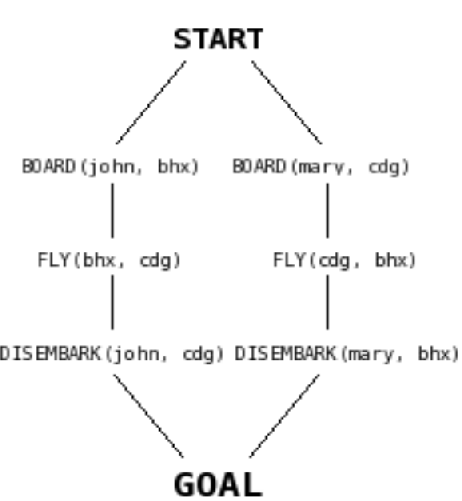
\includegraphics{IntroToAIE2PartialPlan.png}
\end{center}
\subsection{Answer - (d)}
Let the LHS of the plan be x1, x2 and x3 respectively. Similarly, let the RHS of the plan be y1, y2 and y3 respectively. There are four possible placements of our x1/y1 values: \\

$$ x1\ x2\ x3\ y1\ y2\ y3\ $$
$$ y1\ x1\ x2\ x3\ y2\ y3\ $$
$$ x1\ y1\ x2\ x3\ y2\ y3\ $$
$$ x1\ x2\ y1\ x3\ y2\ y3\ $$

Hence, there are also 10 possible places for our x2/y2 values. We subtract 4 from this though, to avoid repetition. Finally, there are twenty possible places for our x3/y3 values. We subtract 10 from this to avoid repetition. This gives us:

$$4 + 6 + 10 = 20$$
Hence, there are 20 total-order plans that can be compiled from our partial-order plan.

\end{document}